\documentclass[../Main.tex]{subfiles}


\begin{document}

%%%%%%%%%%%%%%%%%%%%%% TITLE PAGE %%%%%%%%%%%%%%%%%%%%%%
% \newcommand\nbvspace[1][3]{\vspace*{\stretch{#1}}}
% % allow some slack to avoid under/overfull boxes
% \newcommand\nbstretchyspace{\spaceskip0.5em plus 0.25em minus 0.25em}
% % To improve spacing on titlepages
% \newcommand{\nbtitlestretch}{\spaceskip0.6em}
%
% \begin{titlepage}
% \centering
%
% {
\includegraphics[width=0.2\textwidth]{\ip/logo}\par}
% \vspace{1.0em}
% {\nbtitlestretch\LARGE \textbf{University of Granada}}
%
% \nbvspace[2]
%
% \Large
% \texttt{
% 	Analysis of the\\
% 	Blockchain Protocol\\
% }
%
% \nbvspace[0.25]
%
% 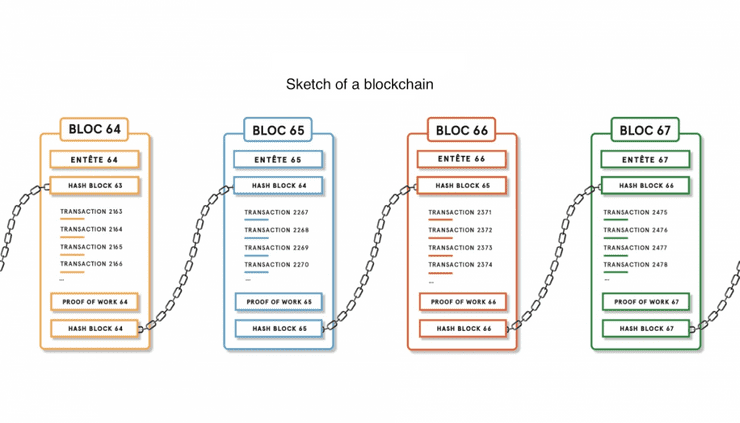
\includegraphics[width=1.0\textwidth]{\ip/title}
%
% \nbvspace[2]
%
% \footnotesize \textbf{Student}\\
% \normalsize Baltasar del Sol de Haro\\[1.0em]
% \footnotesize \textbf{Tutor} \\
% \normalsize Juan Antonio Holgado Terriza\\
%
% \end{titlepage}


\begin{titlepage}
	\AddToShipoutPicture*{\BackgroundPic}
	\phantomsection 
	\pdfbookmark[1]{Título}{title}

	% Para que el título esté centrado en la página.
	% Los valores numéricos deberán elegirse de acuerdo con el diseño de
	% página (sobre todo si se cambia la opción BCOR o DIV).
	\begin{addmargin}[2.575cm]{0cm}
		\begin{flushleft}
			\Large  
			\hfill\vfil

			\large{\textsf{Facultad de ciencias \\ E.T.S Ingeniería Informática y de Telecomunicación}}
			\vfill

			{\large\textsc Doble Bachelor's Degree in Computer Science and Mathematics} \vfill


			{\large\textsc{Final Project}}

			\begin{flushleft}
				\Huge
				\setstretch{0.8}
				A Formal Model to Bitcoin Foundation
			\end{flushleft}

			\vfill\vfill\vfill\vfill

			\textsf{\normalsize{Student:}}\\
			{\normalsize\textrm{Baltasar del Sol de Haro}} 
			\bigskip

			\textsf{\normalsize{Tutor:}}\\
			{\normalsize\rmfamily Juan Antonio Holgado Terriza \\ \emph{Departamento de Lenguajes y Sistemas Informáticos}}

			\bigskip
			\textsf{\normalsize{Year 2022}}
		\end{flushleft}  
	\end{addmargin}       

\end{titlepage}  


%%%%%%%%%%%%%%%%%%%%%%% DEDICATIONS %%%%%%%%%%%%%%%%%%%%%%
\begin{flushright}
	\null
	\vspace{15em}
	\emph{To God, my family and friends.}
\end{flushright}



%%%%%%%%%%%%%%%%%%%%%%%% ABSTRACT %%%%%%%%%%%%%%%%%%%%%%%%
\clearpage
\null
\vfill
\begin{center}
	\textbf{Abstract}
	\vspace{1em}

	The present work strives to present a complete description of a protocol(the Bitcoin protocol) that uses the blockchain technology under the conditions of a formal computational model and analyze its properties in order to solve some two problems, namely the Byzantine Generals problem and the Public Transaction Ledger problem.
\end{center}	
\vfill

\clearpage
\null
\vfill
\begin{center}
	\textbf{Sumario}
	\vspace{1em}

	El presente trabajo tiene como objetivo presentar una description completa de un protocolo(el protocolo Bitcoin) que utiliza la tecnología blockchain en el marco de un modelo computacional formal y el análisis de las propiedades del mismo para resolver dos problemas, el problema de los Generales Bizantinos y el problema de Mantener un Registro de Transacciones Público Distribuido.
	\end{center}	
\vfill

%%%%%%%%%%%%%%%%%%%%%%%%% TABLES %%%%%%%%%%%%%%%%%%%%%%%%%
\setcounter{tocdepth}{1}
\tableofcontents
\listoffigures
\listoftables



%%%%%%%%%%%% TABLE OF SYMBOLS AND NOTATIONS %%%%%%%%%%%%%



%%%%%%%%%%%%%%%%%%%%%%%% PREFACIO %%%%%%%%%%%%%%%%%%%%%%%



\end{document}
